\documentclass[a4paper]{article}

%% Language and font encodings
\usepackage[english]{babel}
\usepackage[utf8x]{inputenc}
\usepackage[T1]{fontenc}

%% Sets page size and margins
\usepackage[a4paper,top=3cm,bottom=2cm,left=3cm,right=3cm,marginparwidth=1.75cm]{geometry}

%% Useful packages
\usepackage{amsmath}
\usepackage{graphicx}
\usepackage[colorinlistoftodos]{todonotes}
\usepackage[colorlinks=true, allcolors=blue]{hyperref}
\usepackage{float}

\graphicspath{ {images/} }

\title{Parallel Tree Search In Playing The Game 2048}
\author{}
% Update supervisor and other title stuff in title/title.tex

\begin{document}
\begin{titlepage}

\newcommand{\HRule}{\rule{\linewidth}{0.5mm}} % Defines a new command for the horizontal lines, change thickness here

\center % Center everything on the page
 
%----------------------------------------------------------------------------------------
%	HEADING SECTIONS
%----------------------------------------------------------------------------------------

\textsc{\LARGE University of the Witwatersrand}\\[1.5cm] % Name of your university/college
\textsc{\Large COMS4040: High Performance Computing and Scientific Data Management Group Assignment}\\[0.5cm] % Major heading such as course name
% \textsc{\large Minor Heading}\\[0.5cm] % Minor heading such as course title

%----------------------------------------------------------------------------------------
%	TITLE SECTION
%----------------------------------------------------------------------------------------
\makeatletter
\HRule \\[0.4cm]
{ \huge \bfseries \@title}\\[0.4cm] % Title of your document
\HRule \\[1.5cm]
 
%----------------------------------------------------------------------------------------
%	AUTHOR SECTION
%----------------------------------------------------------------------------------------
{\large \today}\\[2cm] % Date, change the \today to a set date if you want to be precise

\begin{minipage}{1\textwidth}
  \Large \emph By Mizrahi, M. (708810)\\
  \Large \emph By Chalom, J. (711985)\\
\end{minipage}

% If you don't want a supervisor, uncomment the two lines below and remove the section above
%\Large \emph{Author:}\\
%John \textsc{Smith}\\[3cm] % Your name

%----------------------------------------------------------------------------------------
%	DATE SECTION
%----------------------------------------------------------------------------------------



%----------------------------------------------------------------------------------------
%	LOGO SECTION
%----------------------------------------------------------------------------------------

% \includegraphics[width=8cm]{title/logo.png}\\[1cm] % Include a department/university logo - this will require the graphicx package
 
%----------------------------------------------------------------------------------------

\vfill % Fill the rest of the page with whitespace

\end{titlepage}

% \lfoot{School of Computer Science and Applied Mathematics}
\clearpage
\setcounter{page}{1}
% \setcounter{section}{1}
\pagenumbering{arabic}

\section*{Abstract}
Tree searching for artificial intelligence problems is very computationally intensive in terms of the amount of memory required to construct realistically sized game trees. The nature of how trees work means that sub-trees in seperate sections of the game tree are independant which makes these kinds of trees highly parallelisable. Our MPI implementation is able to scale massively and produced very fast results on large amounts of nodes for the game of 2048. The Cuda implementation is able to build thousands of sub-trees which all execute in lock-step. A single sub-tree is much slower than either serial or MPI in execution but a single Cuda run can beat the other implementation in scale versus total final time. Cuda however has serious memory constraints with the number of sub-nodes of each sub-tree generated whereas MPI's restictions are based on each specific node's specifications.

\section{Introduction}
Games provide an interesting set of problems for artificial intelligence since they provide a level of complexity whilst having clearly defined rules which lends these problems to implementation and simulation. Many games have solution spaces which are intractably large and therefore algorithms and methods employed to solve or approximate any optimal solution to these spaces have to employ smart techniques to deal with the computational constraints of such problems. High performance computing then lends itself to expanding the capabilities of these methods to deal with much larger solution spaces in much shorter amounts of time than a serial approach’s performance could achieve. \cite{AIModern}

\subsection{Problem statement}
We wish to enhance a tree search algorithm by using high performance technologies so that we can improve its performance. The tree search algorithm will be applied to a game called 2048.

\section{Background}
\subsection{The game 2048}
This is a single-player non-deterministic sliding block puzzle game. It’s a fairly simple game with the aim of producing one tile on the board which is equal to 2048. \cite{rules}

\subsection{The Rules of the game:}
	\begin{itemize}
		\item The game is played on a square grid, i.e. 4x4 or 8x8 grid.
		\item Every turn the player will choose a direction for the blocks to move, either up, down, left or right.
		\item Tiles will slide as far as possible until stopped by the edge of the grid or another block. 
		\item If 2 tiles have the same number while colliding then they will combine into a single block and the new value will be the sum of their values.
		\item After each action, a new tile will appear on the grid with a value of 2.
		\item The game is won when a tile with value of 2048 appears on the board. 
	\end{itemize}

\subsection{Game Trees}
The textbook, Artificial Intelligence: A Modern Approach \cite{AIModern} describes game trees as being directed graphs where each node indicates a game state and each edge indicates an action. A list of edges or connected nodes is a path. A game tree is called complete if it contains all possible actions from each possible state. This means that the size of a game tree can be massive and even exceed the available memory resources of the computing system being used. Each divergent path or sub-tree is mutually exclusive from other sub-trees which branch off either before or at the level of the sub-tree this means that these data structures are highly parallelisable. The main issues with trees is their branching factor and how to assign resources in a smart way to handle the exponentially growing number of nodes.

\section{Methodology}
\subsection{General Assumptions}
All drawn diagrams were drawn using \url{http://draw.io/} and charts were made with Microsoft Excel 2013.\\ All results were calculated as an average of running the same experiment six times and calculating the average result.\\
\noindent The system used for empirical analysis, was the wits cluster which is called Hydra. It consists of around 100 nodes where each node has a quad core CPU where three of the cores are exposed to the cluster. Each node also contains two GTX 750Ti GPUS with 2048MB on-board global memory. For our experiments we used 2 cores per node for the serial and the MPI implementations.
Three implementations of tree searching was used. These being a serial C++ approach, a MPI approach and a Cuda GPU-based approach. All three approaches uses the C++11 standard.
In the Cuda approach we assumed that the sub-trees (computed in parallel) are all completed where dead-nodes are just assigned as ‘empty’ type nodes and then ignored.


\subsection{Testing Method}
We built a game supervisor which keeps track of and maintains the game states and rules. This allowed us to make the different tree and tree search implementations consistent in their approach to the problem domain. 
We tested the algorithms and their performance based on the number of nodes in the tree they were able to implement versus the time it took to generate those respective trees for each algorithm. We ran each test several times and took the average result for each configuration.
We also tested the algorithms on three board sizes, namely 4x4, 6x6, and 8x8.


\subsection{Implementation}
All the technologies use some form of the C/C++ programming language and specification. All implementations were designed to use a helper class which contains code which is the same across the three implementations. The three implementations also share a class structure for the tree and the nodes of the tree respectively. We made use of a node and pointer tree implementation. The Cuda implementation makes use of many pre-compiler directives to change the shared function calls into Cuda specific function calls – this was done to try and reuse code as much as possible. Certain functions had to be duplicated and parts modified to fit in the correct specification and paradigm depending on the implementation used.
For both MPI and Cuda our strategy was to initially generate a tree using a serial method which would go to a depth where the number of cut-off states (the states which are not win states or dead-ends) are equal to the scale of parallelism we want – the number of nodes in MPI and the number of threads in Cuda. This meant that we could then treat these cut-off states as their own local roots of their respective sub-trees which we would then generate in parallel on each respective computing device. This strategy worked very well because the number of parallel tree constructions was far smaller than the final number of nodes we were able to generate. We believed that the overhead of parallelising the tree building in a dynamic load balancing manner \cite{parallel}  would be far greater than the cost of a very small initial serial step. This meant that no parallel data communication was needed after each process got their initial node from which to build their respective sub-tree.

\subsubsection{Serial Approach}
	\begin{itemize}
		\item We used a user controlled stack in order to build the tree.
		\item From the root node, all possible children are pushed to the stack.
		\item Then for each node at the top of the stack:
		  \begin{itemize}
		    \item Each child is checked to see if it’s a dead state or if it is a solution state
		    \item A dead state is one where there are no possible moves left.
		    \item If not dead state or solution state then it is pushed to the top of the stack
		    \item If a solution is found then store it for later processing.
		  \end{itemize}
		\item However, since the game tree is so big for 2048, the tree is limited by the number of nodes.
	\end{itemize}

\begin{figure}[H]
	\centering
	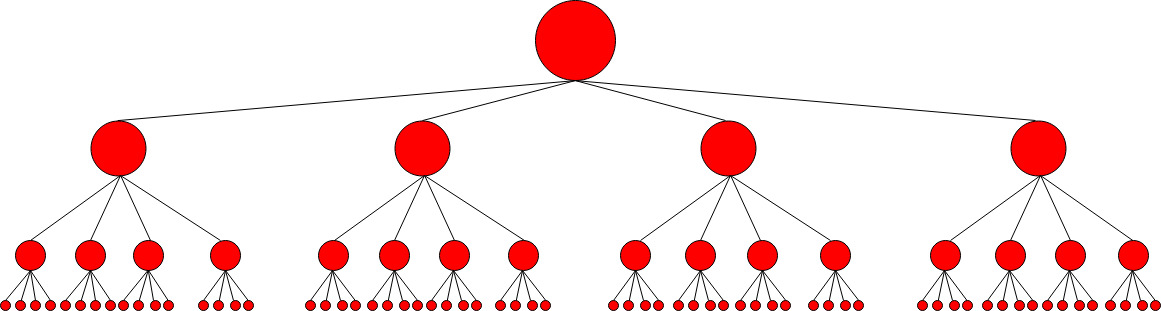
\includegraphics[width=1.0\textwidth,scale=1.0]{images/tree}
	\caption{Tree structure of 2048 in serial approach}
\end{figure}

\subsubsection{MPI Approach}
	\begin{itemize}
		\item The MPI approach is very similar to the serial approach.
		\item The root process creates a small sub-tree until the number of leaves is equal to number of processes used.
		\item Each process is sent its initial state
		\item Each process then creates a serial search from the initial state.
		\item Then each process sends back its local optimal solution depth to the root process.
		\item The root process compares them and chooses the minimum.
	\end{itemize}

\begin{figure}[H]
	\centering
	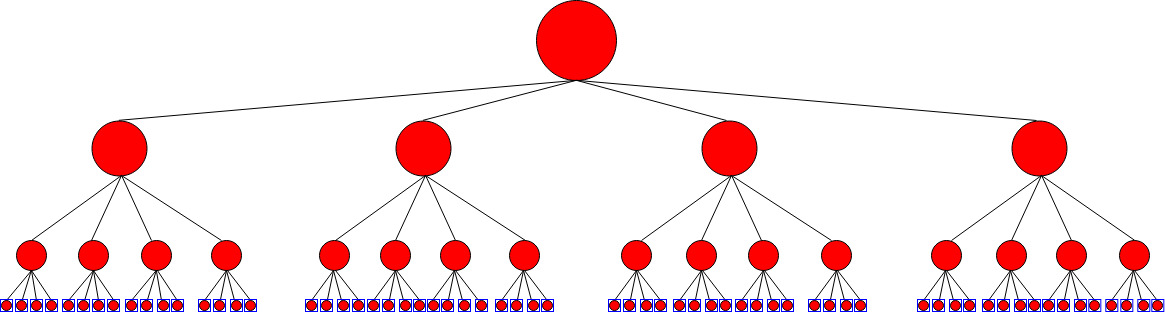
\includegraphics[width=1.0\textwidth,scale=1.0]{images/tree_mpi}
	\caption{Tree structure of 2048 in MPI approach. The leaf nodes are distributed to each process where a serial tree search is run using the leaf nodes as the new root nodes.}
\end{figure}

\noindent The leaf nodes are distributed to each process where a serial tree search is run using the leaf nodes as the new root nodes.

\subsubsection{Cuda Approach}
	\begin{itemize}
		\item The CUDA approach starts in a similar manner to the MPI approach.
		\item The host generates a small sub-tree and stores each initial state to be used by each Cuda thread to generate a sub-tree.
		\item Each thread then creates an array to store its own sub-tree. This array contains the max-number of nodes per sub-tree that has been specified.
		\item For each entry in a thread's sub-tree array, the nodes children are created and placed in the array.
		\item For this approach to work, we must assume the tree is complete and symmetric. An empty node is handled as its own constructir and then ignored when searching back from found solutions.
	\end{itemize}


\begin{figure}[H]
	\centering
	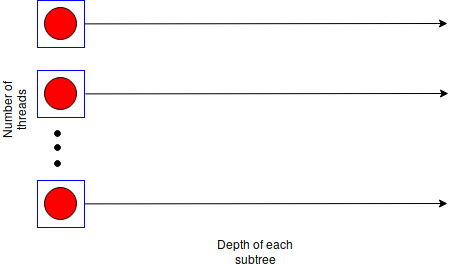
\includegraphics[width=1.0\textwidth,scale=1.0]{images/tree_cuda}
	\caption{Tree structure of 2048 in Cuda approach. The leaf nodes are stored in an array where the first column has the initial states for each thread and each row represents a subtree to be explored.}
\end{figure}

\noindent A down side with the Cuda implementation is that we were unable to perform a warm-up step – beyond initialising the cuRand library - as that would mean building the entire tree twice.

\section{Experimental setup}
Since the game 2048 is a single player game we were able to independently run each AI and then analyse the returned results. Each AI kept track of certain statistics such as number of nodes and the time taken to reach a tree of each node size. We also built many command line parameters into the AI programs so that we could change the parameters and dynamics of the domain and AI at will. We used these parameters to test a variety of node sizes from 10000 nodes up to 5000000 nodes and to change the board size as needed. For the MPI implementation we also changed the number of processor nodes from the cluster that we used so that we could analyse the results to determine how the different node configurations effected performance. \\

\noindent We would start each AI with an initial state which would be generated using a pseudo-random number generator and scheme. We could choose to seed the PRNG with a static value to force the same initial state across our implementations.\\

\noindent We used the PBS scripts to allow us to repeat each experiment (with a precise configuration) many times to get a more accurate result. Each AI was capable (via the helper functions we made) to save their results as csv files which we were then able to open in Excel to process and generate graphs for each implementation’s performance. 


\section{Results and discussions}

\subsection{Charts}


\begin{figure}[H]
	\centering
	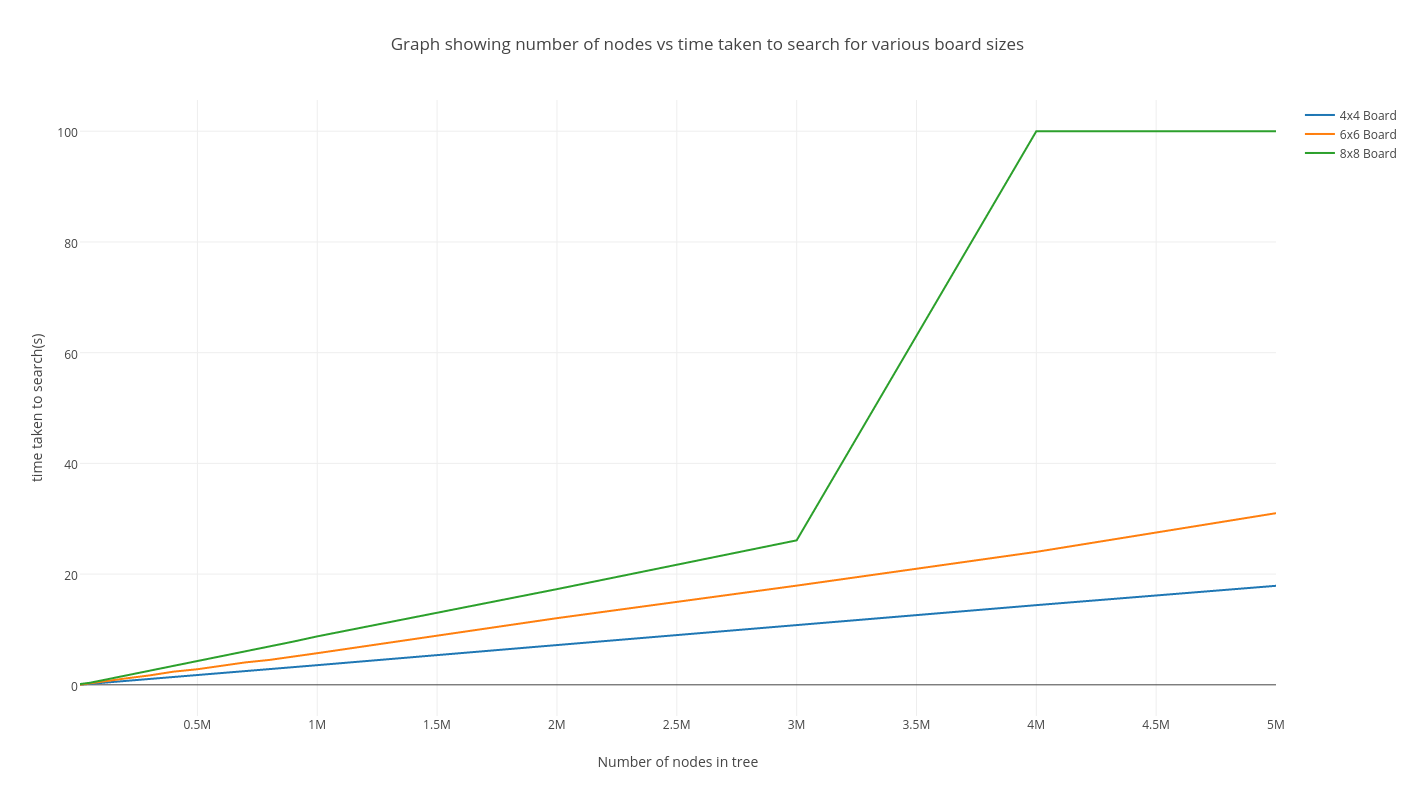
\includegraphics[width=1.0\textwidth,scale=1.0]{images/serial_graph}
	\caption{Serial execution time}
\end{figure}

\begin{figure}[H]
	\centering
	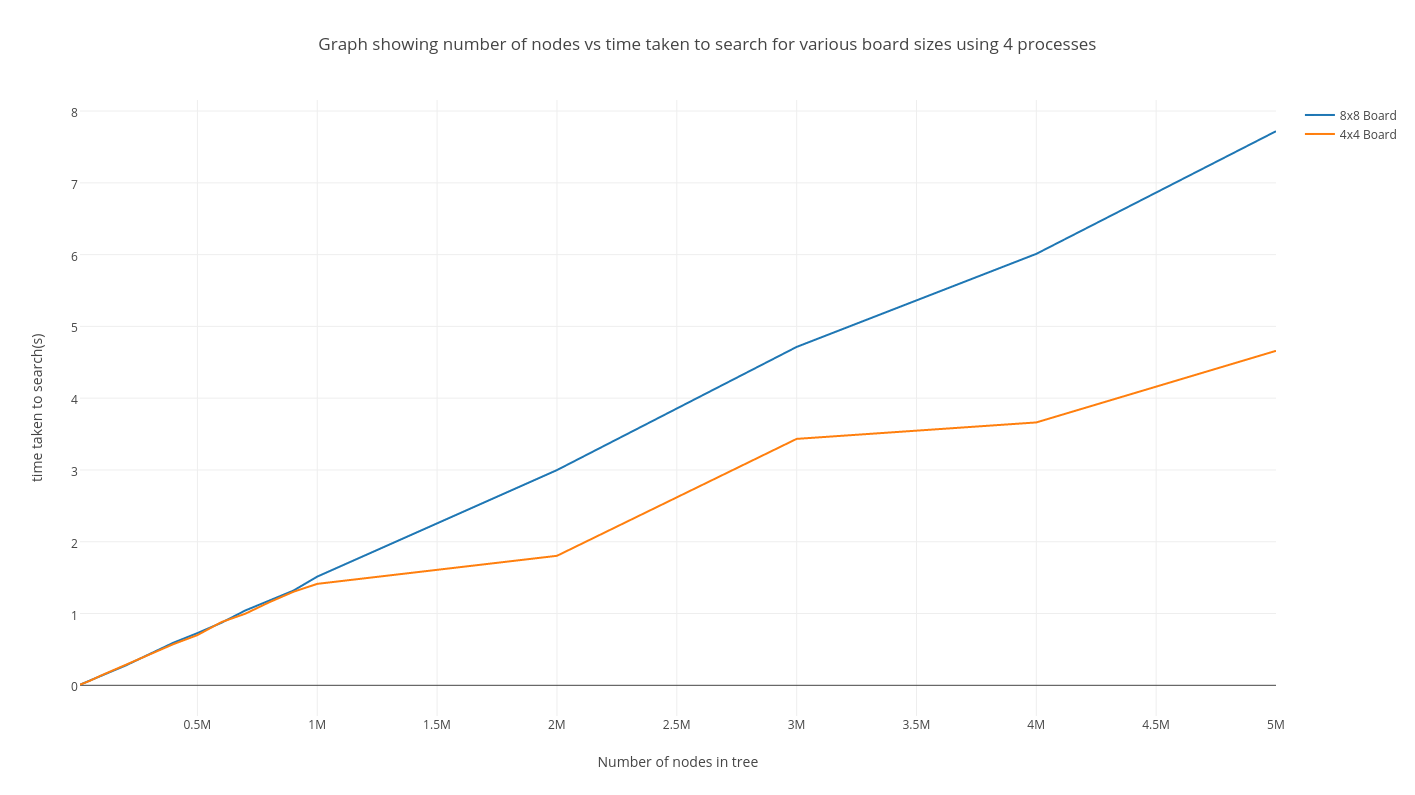
\includegraphics[width=1.0\textwidth,scale=1.0]{images/mpi_4procs}
	\caption{MPI execution time where number of nodes is divided by 4 processes evenly}
\end{figure}

\begin{figure}[H]
	\centering
	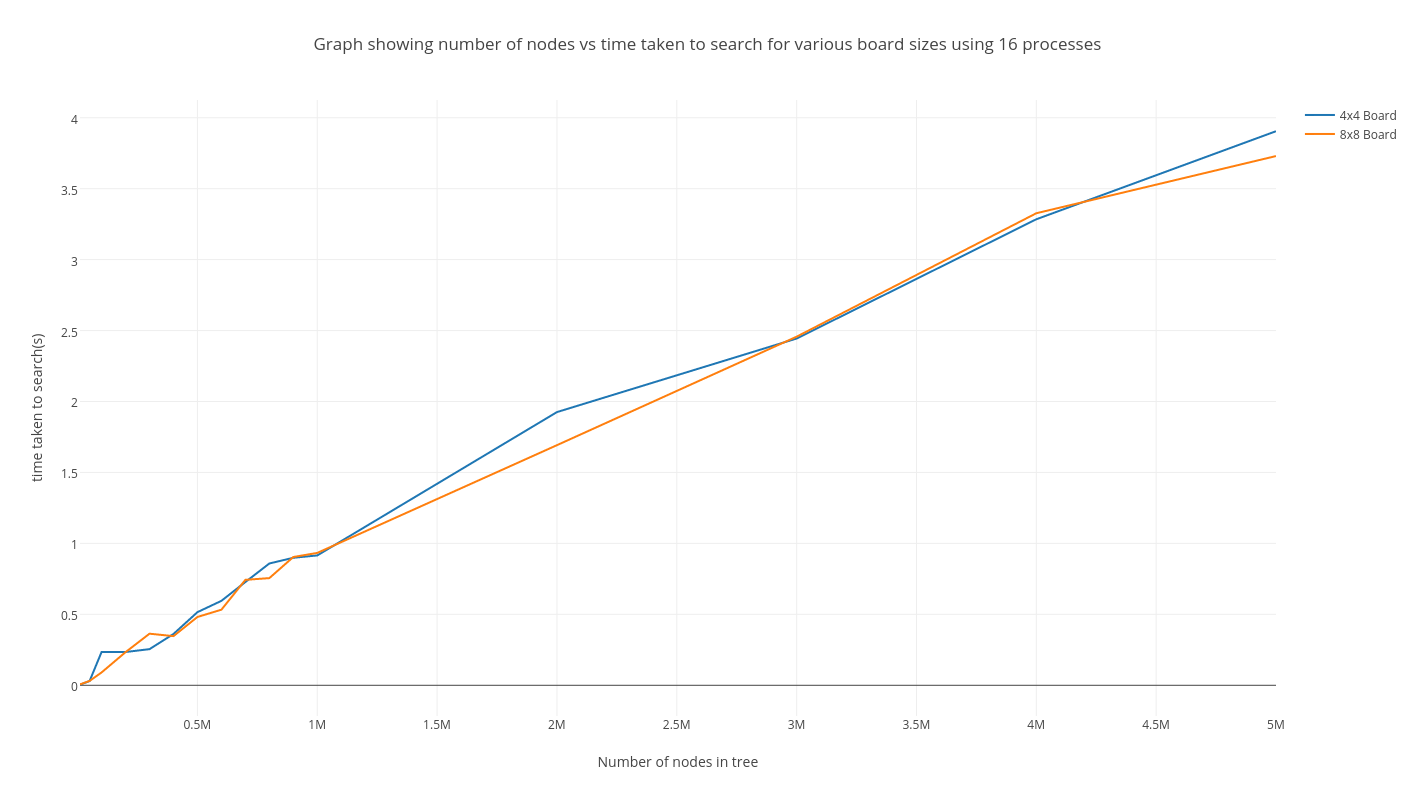
\includegraphics[width=1.0\textwidth,scale=1.0]{images/mpi_16procs}
	\caption{MPI execution time where number of nodes is divided by 16 processes evenly}
\end{figure}

\begin{figure}[H]
	\centering
	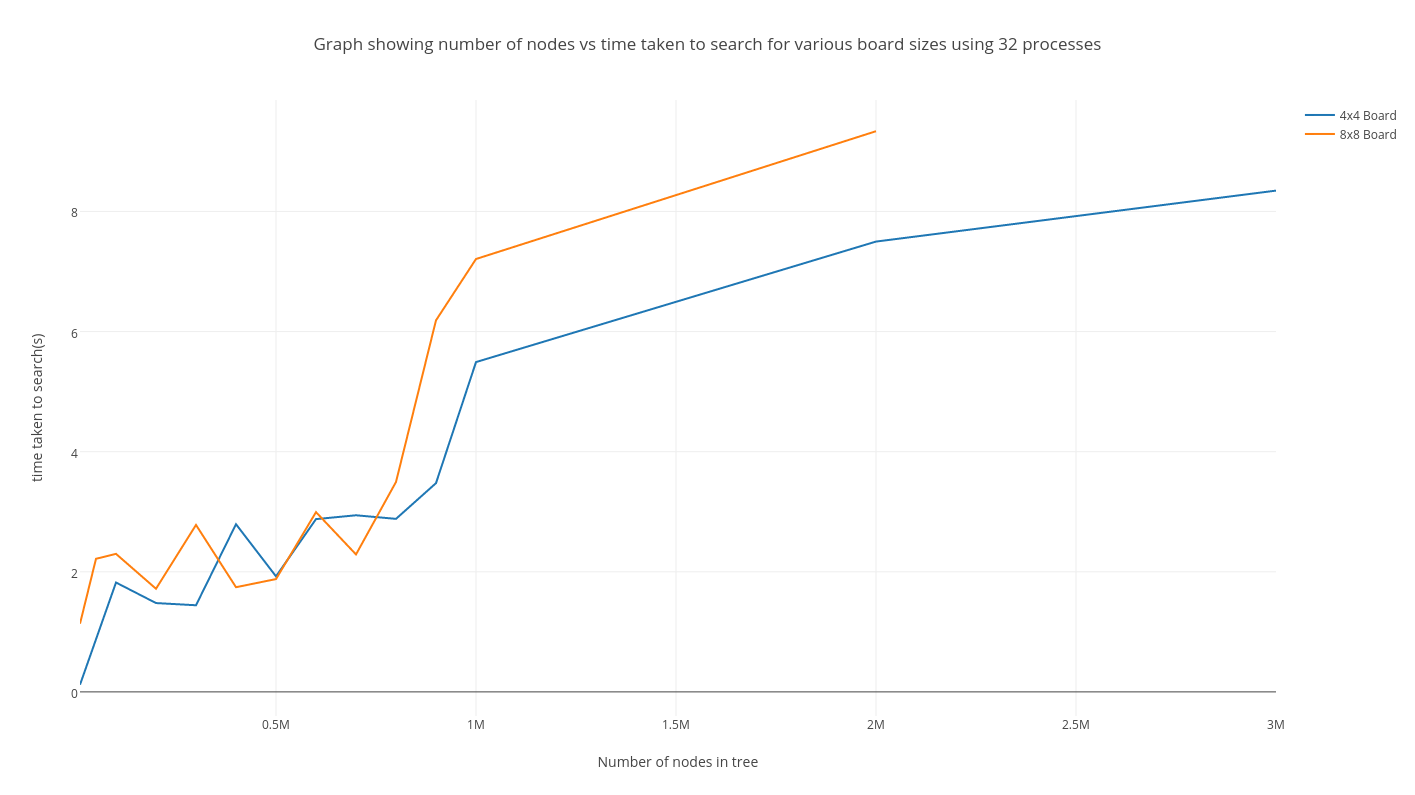
\includegraphics[width=1.0\textwidth,scale=1.0]{images/mpi_32procs}
	\caption{MPI execution time where number of nodes is divided by 32 processes evenly}
\end{figure}

\begin{figure}[H]
	\centering
	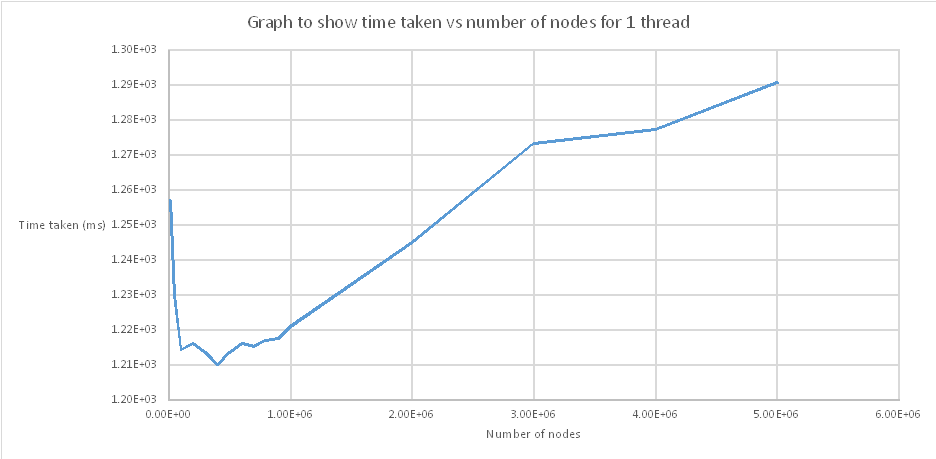
\includegraphics[width=1.0\textwidth,scale=1.0]{images/cuda_1thread}
	\caption{Cuda execution time for 1 thread}
\end{figure}

\begin{figure}[H]
	\centering
	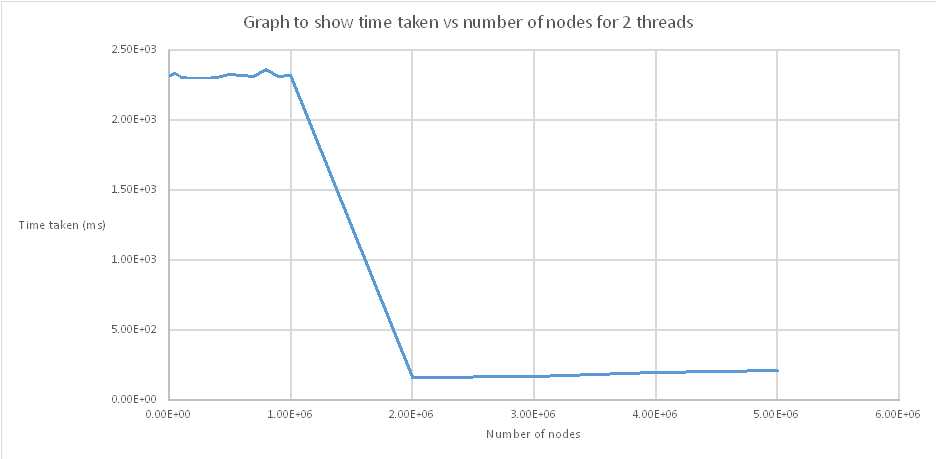
\includegraphics[width=1.0\textwidth,scale=1.0]{images/cuda_2threads}
	\caption{Cuda execution time for 2 threads}
\end{figure}

\begin{figure}[H]
	\centering
	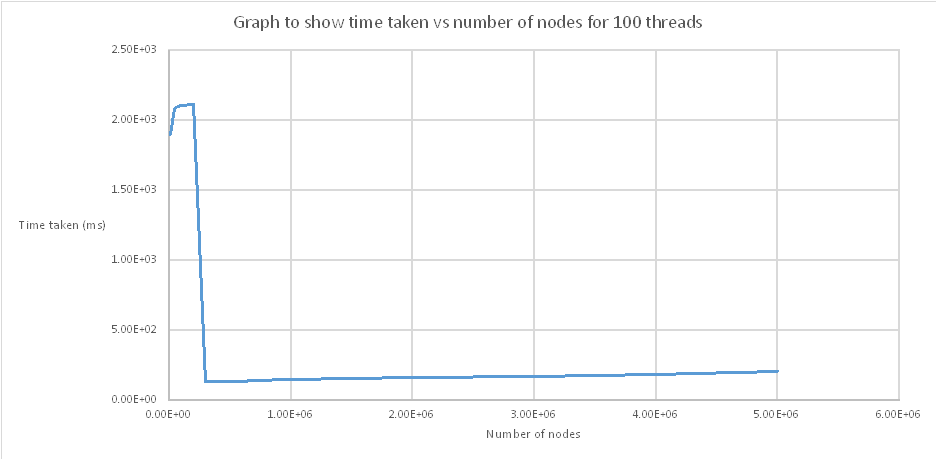
\includegraphics[width=1.0\textwidth,scale=1.0]{images/cuda_100threads}
	\caption{Cuda execution time for 100 threads}
\end{figure}


\begin{figure}[H]
	\centering
	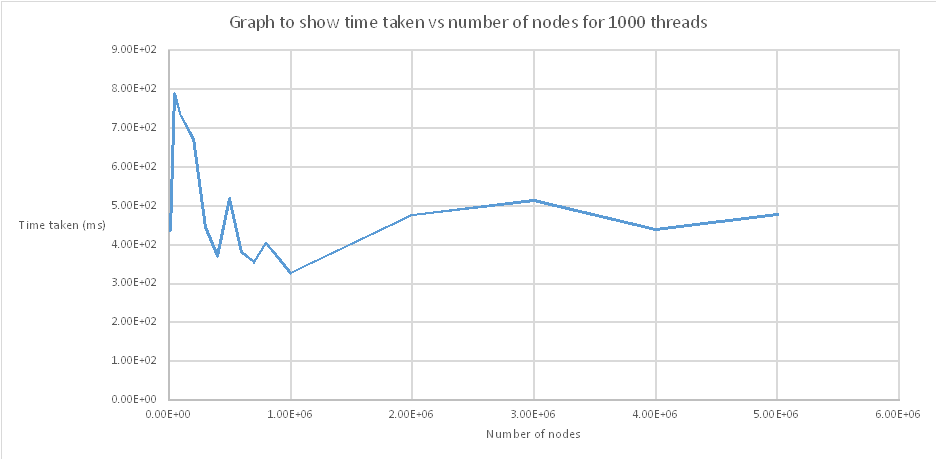
\includegraphics[width=1.0\textwidth,scale=1.0]{images/cuda_1000threads}
	\caption{Cuda execution time for 1000 threads}
\end{figure}


\subsection{Discussion on performance of results}
Using the serial algorithm on the cluster and using anything over 3 million nodes resulted in the program being killed as there was too much computation for one process to do. From our results we found that increasing the board size produces a linear increase in time. In the serial implementation, 5 million nodes on a 4x4 board took 17.882812 seconds, while using MPI with 4 processes resulted 4.659657 seconds. This means there is a speedup of 3.838. Using MPI with 16 processes and the same setup resulted in 3.904706 seconds. This means there is a speedup of 4.580.
The results for using 32 processes resulted in haphazard timing for a low number of nodes. This could be due to each process doing a very little amount of work and as such the problem size should be increased to keep the same efficiency as using 4 processes and 16 processes. 

The Cuda results show a spike in times when the work required is very little. When the work size is increased the graphs tend to stabilize and show a linear relationship between the time taken and the number of nodes.

\noindent By running the serial algorithm using increasing board sizes, we found that as the board size is increased the percentage of leaf nodes that are solutions also increases. When usig a 4x4 board, only 12\% of the leaves are solutions.However, using a 16x16 board, 99\% of the leaves are solutions. This could be due to the increased space which allows for more correcting of mistakes and hence less states to be trapped in.

\subsubsection{Complexity Analysis}
Because the tree is asymmetric, the exact size of the tree cannot be determined. If we assume that the tree is complete then there would be $4^n$ nodes, where $n$ is depth of the search. We found that the minimum depth is always around 1000. This means that is the tree were complete then there would be $4^1000$ nodes. 

\subsection{Problems we encountered with this project}
We had many problems in this project and found solutions or workarounds to a lot of these problems.\\

\noindent We initially attempted to implement an in-place depth-first-search because we believed that it would be more memory efficient than either a recursive or user-managed stack approach. We found that the implementation was difficult and ended up changing our implementation to a user-managed stack.\\

\noindent We thought that we would be able to search the entire game tree for 2048 but it turns out that it is a very large game tree. This game tree is also asymmetric which makes it unlikely for the size of any given game tree to be accurately determined. We had to change our project slightly so that our AIs would only search a sub-tree from any initial state and then return a local minimum path from that search.\\

\noindent We initially used strings to represent our game state. Cuda does not support strings and we had issues managing states. We fixed this by moving to an array of ints.
Attempting to code in a way which reduced redundant code for three different paradigms was difficult and sometimes impossible. We ended up having some forced redundancy when certain functions or methods were incompatible with one of our implementations, namely Cuda.\\

\noindent The Cuda implementation was the most challenging part of the project. Cuda is not very well documented and every new generation of GPU introduces new features and quirks. We worked on the 700 series which has now become deprecated. This means that ways of doing things which are now supported were not for us. A big issue is that Cuda does not like nested data in classes and will not copy such data from the host to the device or vice versa. Random number generation was also difficult because the cuRand library does not follow the same conventions as the main parts of the Cuda run-time, such as returning errors. The final issue we had was that indexing was very difficult because we had to flatten our class structure and use primitive 1D arrays where possible. We spent lots of time figuring out how our indexes worked. What we had to do in the end is flatten our data structures and only give the device each initial game board we had computed in serial. The GPU would then generate in device global memory each sub-tree (per thread) and return only the most optimal path and its respective thread. We know how many nodes were generated because we had to assume that the tree was complete and any node which was a dead-end became an empty node.\\

\noindent The cluster’s restrictions killed the serial AI when it was busy executing 4000000 and 5000000 nodes.


\section{Conclusion}
From our experimentation we found that using MPI, we can get a massive speed performance by distributing the work across multiple processes. The extension from the serial algorithm to the MPI algorithm was very simple and did not require too much extra work. However, Cuda requires special attention when adapting the serial algorithm. It requires a lot more work and refactoring of code to suit the Cuda environment, We found that even though Cuda may be slower per subtree, its scalability could potentially be much higher than that of MPI. With efficient use of memory each block would be able to do a lot more work. Overall we found that if there is a task which needs to be repeated but makes use of a lot of memory then MPI woould be a better choice to use. However, if the task is just computationally expensive while not being too memory intensive then Cuda would most likely be a much better choice in parallelisation of the task.



\section*{Acknowledgements}
We made use of the CUDA 8.0 SDK and its associated images and sample programs. We also used the lab examples from class as a way to figure out how to implement CUDA. We would like to thank Dr Richard Klein for his help with the Cuda implementation.

\bibliographystyle{plain}
\bibliography{biblio}{}

\end{document}